\section{Complexity}

Let $M$ x $N$ be the dimension of the video frames, $T$ be the lngth of the video sequence in frames, and $s$ be the width of the spatial neighborhood, and $w$ be the width of the temporal neighborhood. The original formulation of our problem has two variables: the labels $X$ and the edge weights $W$. There is a label for each pixel in the video sequence making $M N T$ label variables. There are $(2 w+1)^2$ weights for each pixel but no weights for the final frame, making $M N (T-1) (2 w + 1)^2$ weight variables. Therefore the original problem has a total of $M^2 N^2 T (T-1) (2 w + 1)^2$ variables. The momentum constraint has a term of the form $W_{ijt}^{ab} |c + \sum K W_{i^{'} j^{'} t+1} |$ which is non-convex, as can be shown by considering the trival example of $W_{ijt}^{ab} = 0.5$ and exactly one of the summed weights $= 0.5$ and testing the convexity condition. Thus the original problem is a quadratic program with a non-positive semidefinite quadratic term $Q$ and is NP-hard \cite{sahni1974computationally}.

Our primal decomposition method finds only an approximate solution to this problem by alternating between solving for the labels and weights using the Horn-Schunk first-order approximation of the imaging function as well as an approximation of the momentum term. With these changes both subproblems are convex.

First we consider the complexity of solving for the labels given the flows without the Horn-Schunk approximation. This problem has $M N T$ variables, but cannot be solved quickly in its raw form. For this reason we convert the problem to epigraph form, introducing $M N T$ new variables for spatial coherence and $M N T (2 w + 1)^2$ variables for temporal coherence. Therefore our total number of variables is $2 M N T + M N T (2 w + 1)^2$, which is typically dominated by the window term $N_{labels} \approx M N T (2 w + 1)^2)$. Since this is a linear integer programming problem it can be solved in order $O((M N T (2 w + 1)^2)^3)$ time. With the Horn-Schunk approximation the $(2 w + 1)^2$ term drops out, leading to $O((M N T)^3)$ solution time.

For solving the flows given the labels, the problem is considerably more difficult to solve with only the momentum approximation. There are $M N T (2 w + 1)^2$ variables to start with, but to put the problem in epigraph form we need to add $2 M N T (2 w + 1)^2 + 2 M N T + 2 M N T (2 w + 1)^2$ variables. This leads to a linear program which can be solved in 
$O((5 M N T (2 w + 1)^2)^3)$ time. With the Horn-Shunk approximation, all of our terms with $(2 w + 1)^2$ drop out, leading to $O((M N T)^3)$ time.

We empirically measured the time to find a solution along each of the dimensions $M, N, T$, and $w$. For simplicity we considered only square images. Figure ~\ref{fig:TimeVsIm} shows the time cost to solve versus the image dimension. We see that increasing the image dimension by a factor of 1.5 from 16x16 to 24x24 leads to a nearly 14x increase in solution time. Similarly in Figure ~\ref{fig:TimeVsLength} we see that the time to solve increases less dramatically, with the cost appearing almost linear. We suspect that this is because the problem size is small enough that the time to build the constraints actually dominates the solution time. Finally in Figure ~\ref{fig:TimeVsWin}, we see that the cost to solve increases dramatically with increased window size, as expected.

\begin{figure}[h]
\begin{center}
	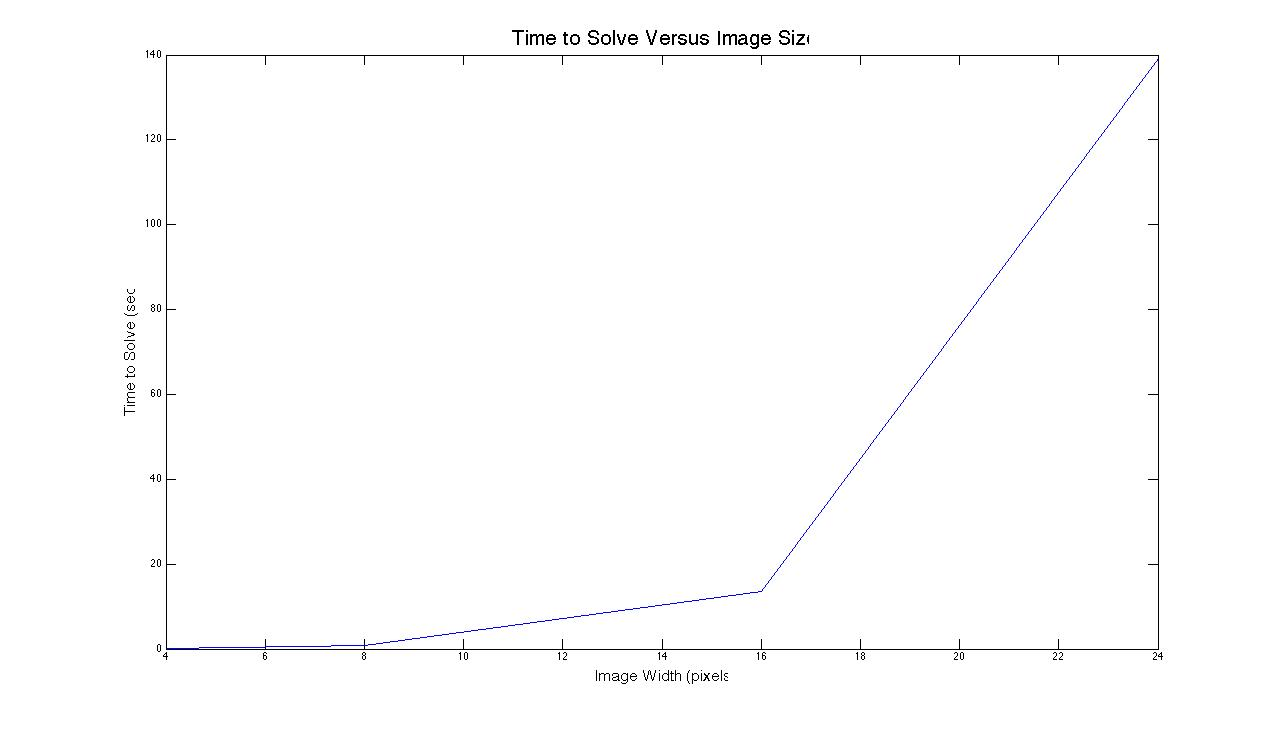
\includegraphics[width=0.45\textwidth, height=2in]{figures/time_vs_imsize.jpg}
	\caption{Time to Solve versus Image Dimension}
	\label{fig:TimeVsIm}
\end{center}
\end{figure}

\begin{figure}[h]
\begin{center}
	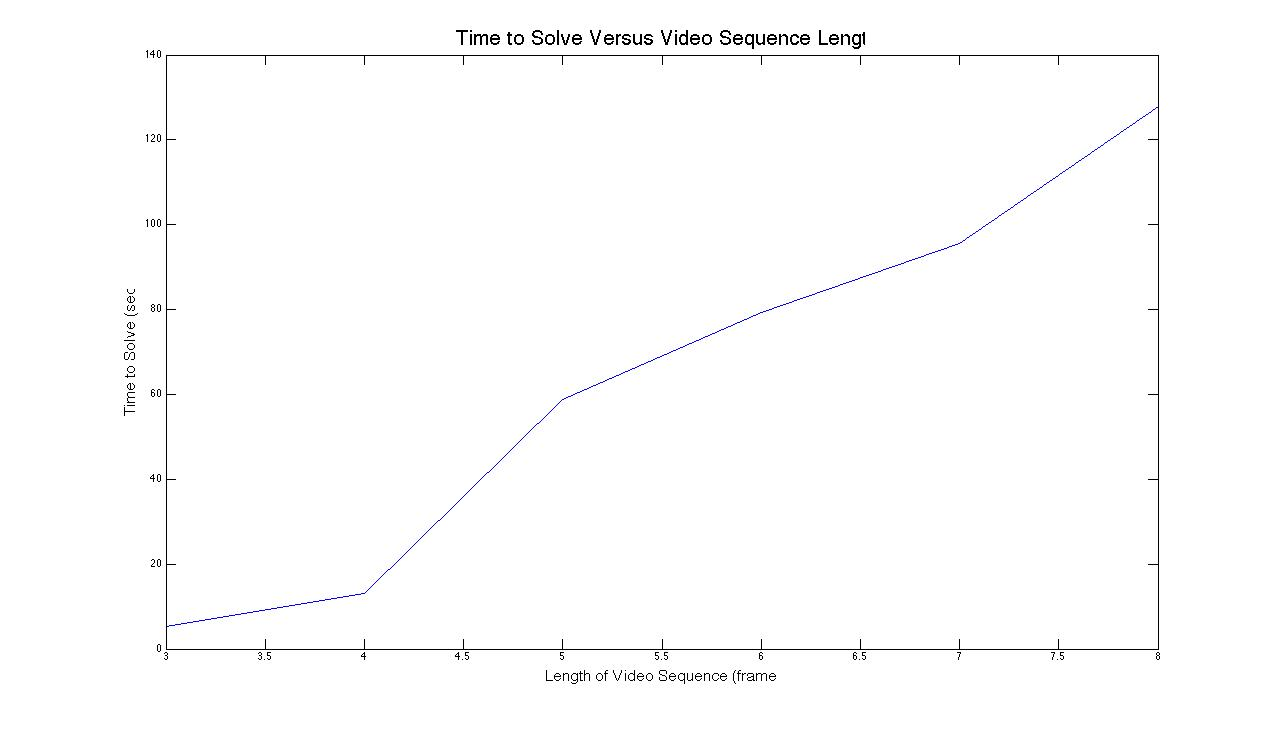
\includegraphics[width=0.45\textwidth, height=2in]{figures/time_vs_length.jpg}
	\caption{Time to Solve versus Sequence Length}
	\label{fig:TimeVsLength}
\end{center}
\end{figure}

\begin{figure}[h]
\begin{center}
	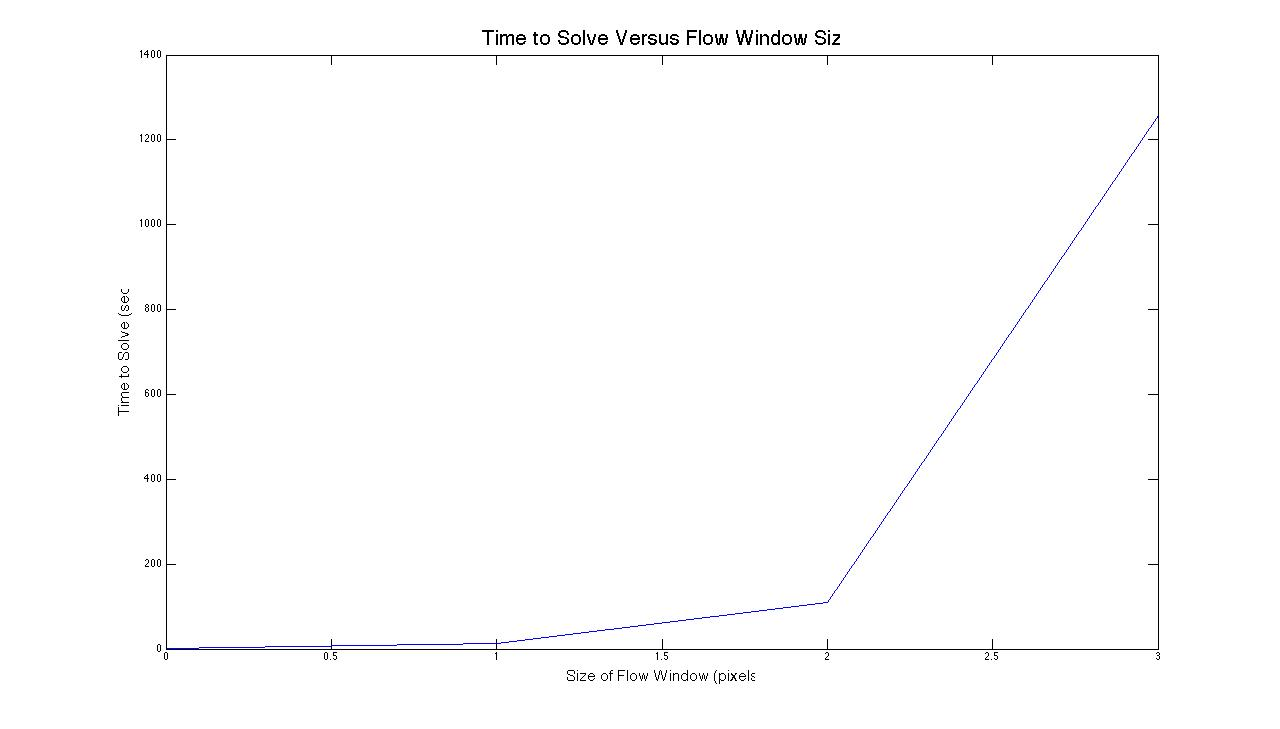
\includegraphics[width=0.45\textwidth, height=2in]{figures/time_vs_window.jpg}
	\caption{Time to Solve versus Window Size}
	\label{fig:TimeVsWin}
\end{center}
\end{figure}